\documentclass[../main.tex]{subfiles}

% DOCUMENT

\begin{document}

\chapter{Giới thiệu}\label{introduce}


Thuộc họ các bài toán tìm đường đi có thời gian đến nhỏ nhất (MATP), phương pháp đầu
tiên được phát triển để giải quyết vấn đề này dựa trên thuật toán
Bellman-Ford trong hai bài báo \cite{bellman1958routing,ford2010flows} và được mô tả bởi
bài \cite{cooke1966shortest} của tác giả Cooke và các cộng sự. Tổng quan về các phương pháp giải khác cho biến thể
này được đề cập trong \cite{dean2004shortest} với lý thuyết về sử dụng mạng FIFO. Đây cũng là một thuộc tính quan trọng sẽ sử dụng trong bài luận.

Bài toán tìm đường đi thời gian tối thiểu (MDP) được nghiên cứu trong bối cảnh mạng lưới giao thông (\cite{demiryurek2011online}), thậm chí trong phân tích mạng xã hội (\cite{gunturi2012information}).

Trong \cite{boland2017continuous} có giới thiệu thuật toán khám phá rời rạc động (DDD) để giải quyết bài
toán tối thiểu hóa chi phí cho mạng dịch vụ theo thời gian liên tục,
thông qua việc sử dụng các biểu thức quy hoạch nguyên trên mạng thời
gian. Giải pháp ở đây là tìm ra các \textbf{thời điểm thích hợp nhất},
cho chúng đi qua các hàm tính toán theo tuần tự nhất định để tạo ra mạng
thời gian từng phần (TEN). Các mạng này được thiết kế để luôn tồn tại nghiệm là đường đi, tìm
ra một giới hạn kép (cận trên và dưới) cho giá trị tối ưu của thời gian
liên tục. Sau khi tìm được tập thích hợp (số ít các thời điểm xác định), mô hình
quy hoạch nguyên sẽ cho ra kết quả tối ưu.


Phần mô tả bài toán, phương pháp giải quyết và kết quả từ khu vực Atlanta của khoá luận 
tham khảo từ bài báo \cite{he2022dynamic}.
Để phục vụ cho các phần sau, dưới đây là một số định nghĩa được sử dụng: 
\begin{itemize}
  \item \textbf{Cây đường đi ngắn
nhất (Shortest-path tree):} Cho đồ thị \(G=(V,E)\), một cây gốc \(s\)
(\(s\in V\)) trong đó nút \(v\) (\(v\in V\)) thuộc cây thì đường đi từ
nút gốc \(s\) đến nút \(v\) luôn là đường đi ngắn nhất.
  \item \textbf{FIFO:} 
  Được lấy từ mạng FIFO trong \cite{dean2004shortest}: 
  đường đi từ \(s\) đến \(v\) là FIFO nếu với mọi cạnh \((u, v)\) trên đường đi, 
  thời gian bắt đầu di chuyển từ \(u\) đến \(v\) không nhỏ hơn thời gian bắt đầu di chuyển 
  từ \(s\) đến \(u\).
\end{itemize}

\section{Mô tả bài toán}\label{problem-description}

Cho một đồ thị có hướng 
\[
  D = (N, A)
\] 
trong đó: \(N = {1, 2, ..., n}\)
là tập đỉnh, \(A \subseteq N \times N\) là tập cạnh; khung thời gian
\([0, T]\) và các hàm vận tốc tuyến tính từng khúc
\(c_{i,j}(t) > 0\) với \(t \in [0, T]\) thỏa mãn tính chất FIFO cho mọi
cạnh \((i, j) \in A\).\\
Tính chất FIFO, trong hàm tuyến tính, nghĩa là
\textbf{độ dốc của các khúc lớn hơn hoặc bằng \(-1\).} 

Không mất tính tổng
quát, ta luôn đi từ đỉnh nguồn \(1\) và kết thúc ở đỉnh đích
\(n\). Đường đi
\[
  P=((i_1^P, t_1^P), (i_2^P, t_2^P), \dots, (i_{m(P)}^P, t_{m(P)}^P))
\]
là một dãy gồm \(m(P)\) nút (cặp đỉnh - thời gian), trong đó dãy các đỉnh
\((i_1^P, i_2^P, \dots, i_{m(P)}^P)\) tạo thành đường đi trong đồ thị
\(D\) từ \(i_1^P\) đến \(i_{m(P)}^P\), và mỗi nút\footnote{Tuy đỉnh và nút có nghĩa tương đồng, nhưng ở đây sẽ quy ước \emph{đỉnh} là một số, \emph{nút} là cặp (đỉnh, thời gian)} trong dãy \(i_k^P\)
tương ứng với thời gian \(t_k^P\), đại diện cho thời gian bắt đầu di
chuyển trên cạnh \((i_k^P, i_{k+1}^P)\) với \(k=1, \dots m(P)-1\). Riêng
đỉnh \(i_k^P\) với \(k=m(P)\) biểu diễn thời gian đến đích. Do đó dãy
các nút cần thỏa mãn tính chất:
\[t_{k+1}^P \ge t_k^P + c_{i_k^P, i_{k+1}^P}(t_k^P)\] với
\(k=1, \dots m(P)-1\). \\
Nếu
\(t_{k}^P \ge t_{k-1}^P + c_{i_{k-1}^P, i_{k}^P}(t_{k-1}^P)\) với \(k \ge 2\) bất kì (hoặc \(t_1^P > 0\) nếu \(k=1\)), thì ta nói rằng đỉnh \(i_k^P\)
cần phải \textbf{đợi}.\\ 
Nếu \(t_{k}^P = t_{k-1}^P + c_{i_{k-1}^P, i_{k}^P}(t_{k-1}^P)\) với mọi
\(k \ge 2\) thì ta nói rằng \(P\) không có chờ đợi (waiting-free). \\
Nếu \(P\) bắt đầu tại đỉnh \(i_1^P = 1\) với \(t_1^P\ge0\) và kết thúc tại
đỉnh \(i_{m(P)}^P=n\) với \(t_{m(P)}^P \le T\) thì ta nói \(P\) là một
đường đi khả thi. Ta kí hiệu \(\mathcal{P}\) biểu diễn tập hợp tất cả các
đường đi khả thi như vậy.

Hai hàm mục tiêu chính được quan tâm ở đây là:

\begin{enumerate}
\def\labelenumi{\arabic{enumi}.}
\tightlist
\item
  \textbf{Tối thiểu thời gian đến đích:}
  \[\min_{P\in \mathcal P}t_{m(P)}^P\]
\item
  \textbf{Tối thiểu thời gian thực hiện (đi từ nguồn đến đích):}
  \[\min_{P\in \mathcal P}(t_{m(P)}^P-t_1^P)\]
\end{enumerate}

Trong phần còn lại của khóa luận sẽ bỏ đi phần chữ \(P\) ở trên các đỉnh cùng một đường đi để thuận tiện cho ký hiệu và dễ nhìn
hơn.

Để minh họa hai hàm mục tiêu này, hãy xem xét đồ thị \autoref{fig:1a} và các hàm vận tốc 
\autoref{fig:1}(b,c,d), với \(n = 3\) và khung thời gian
là \([0, 4]\).

\begin{itemize}
\tightlist
\item
  \textbf{Đường đi tối thiểu thời gian đến đích} là
  \(((1, 0), (3, 3.5))\): Xuất phát tại thời điểm \(t = 0\), đi qua cạnh
  \((1, 3)\) và đến đích tại \(t = 3.5\), giá trị hàm mục tiêu là
  \(3.5\).
\item
  \textbf{Đường đi tối thiểu thời gian thực hiện} là
  \(((1, 1.5), (2, 3), (3, 4))\): đường đi bắt đầu từ \(t = 1.5\), đi
  qua cạnh \((1, 2)\) và đến đỉnh \(2\) tại \(t = 3\). Sau đó bắt đầu từ
  \(t = 3\), đi qua cạnh \((2, 3)\) và đến đỉnh đích tại \(t = 4\), giá
  trị mục tiêu là \(2.5\). Vì không phải chờ đợi trên đường đi này nên
  tổng thời gian di chuyển cũng là \(2.5\).
\end{itemize}

\begin{figure}[h]
\centering
% 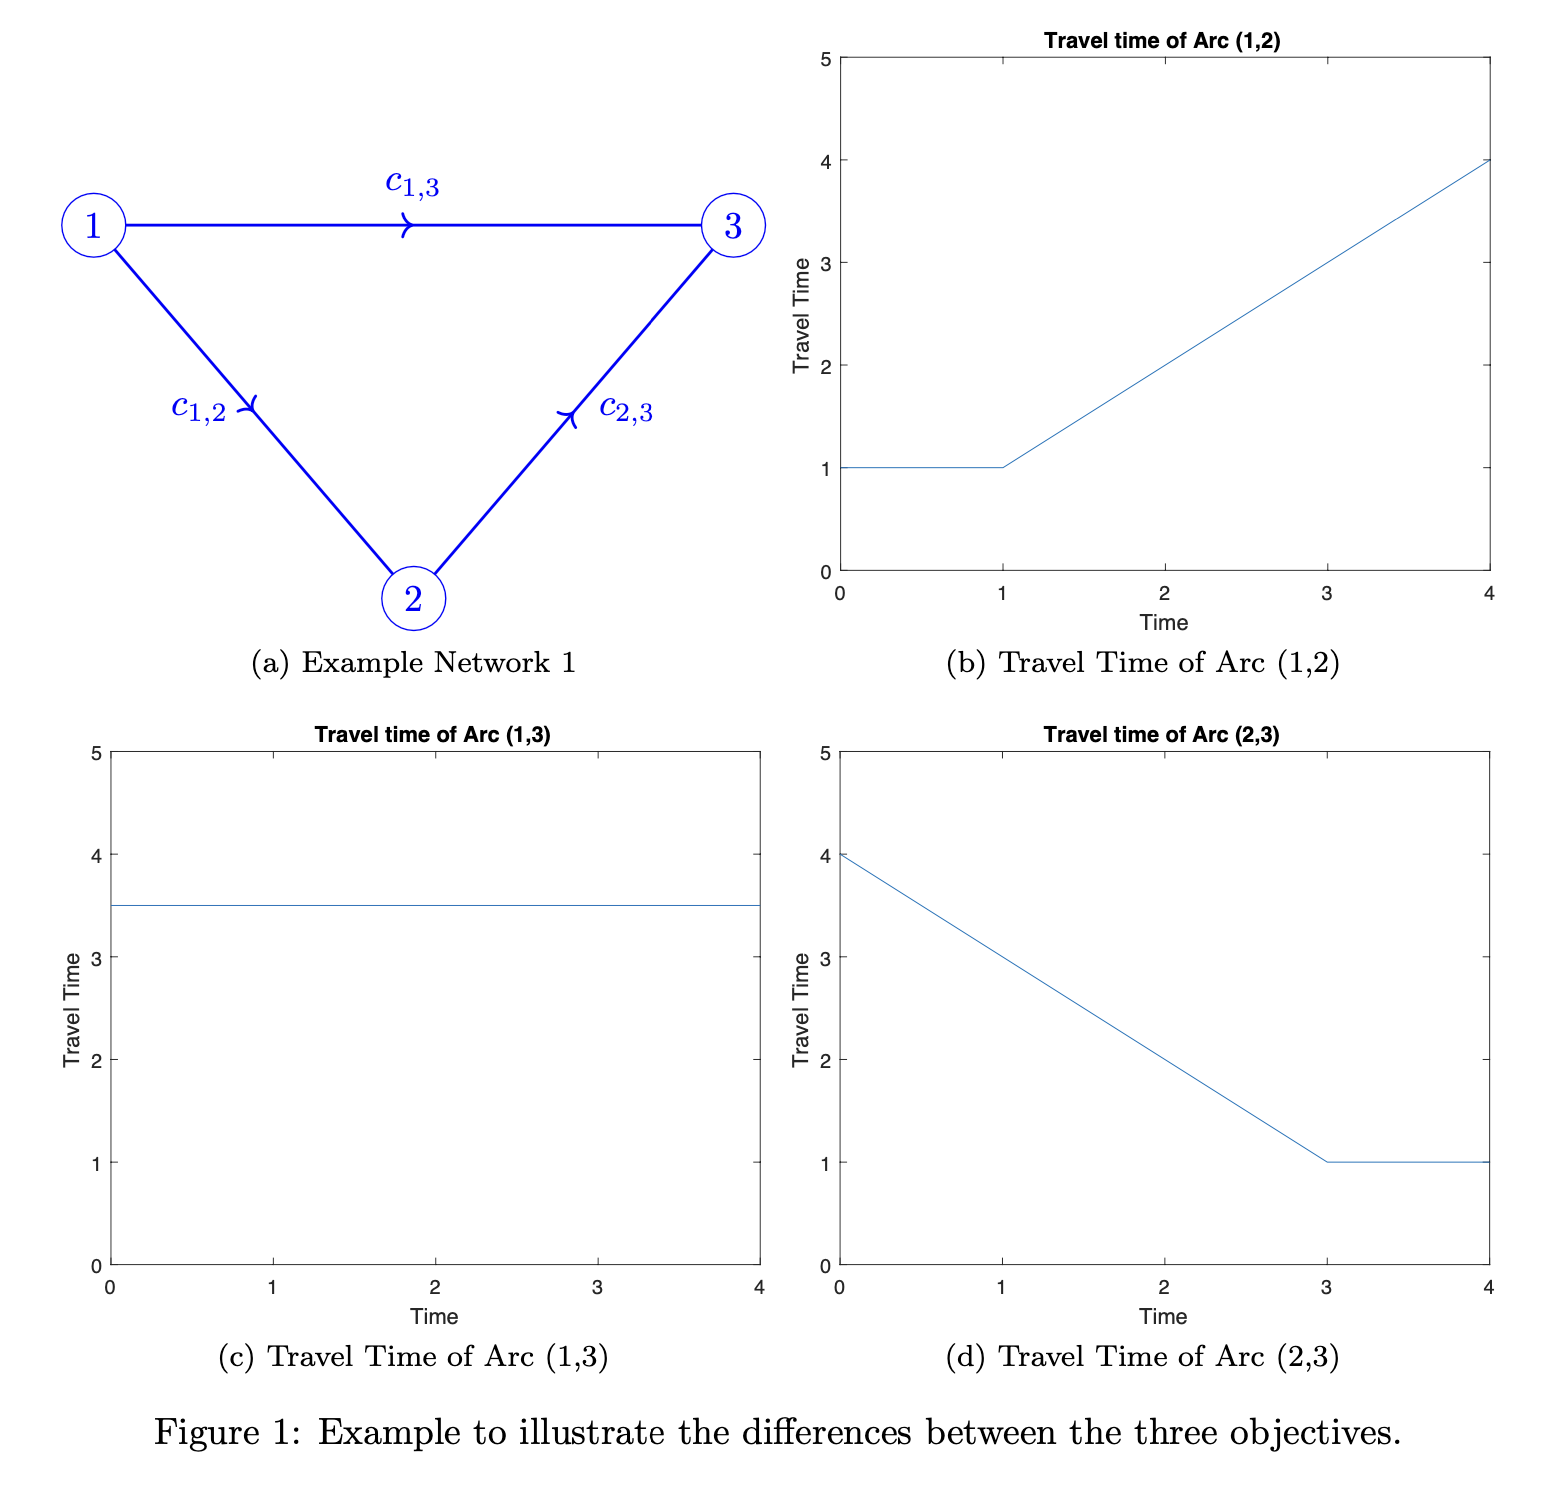
\includegraphics{images/Figure1.png}
\subcaptionbox{Mạng lưới \(1\)\label{fig:1a}}{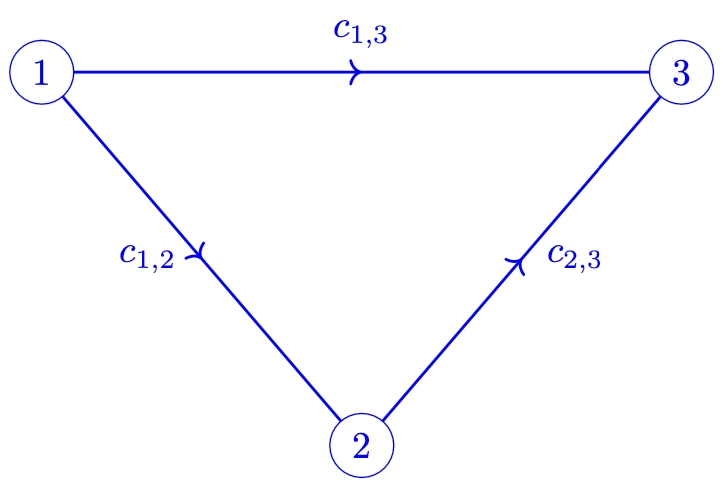
\includegraphics[width=.45\textwidth]{edited-images/Figure1a.jpg}}
\subcaptionbox{Cung \((1, 2)\)\label{fig:1b}}{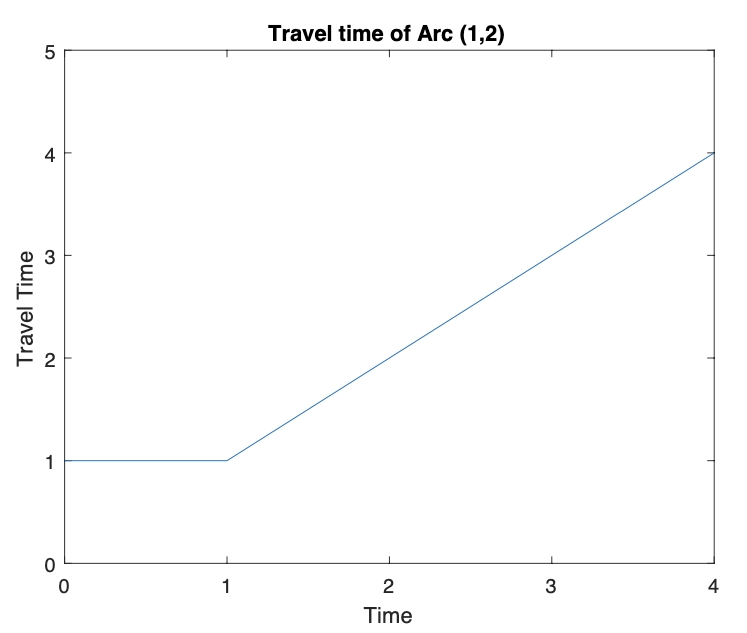
\includegraphics[width=.45\textwidth]{edited-images/Figure1b.jpg}}
\subcaptionbox{Cung \((1, 3)\)\label{fig:1c}}{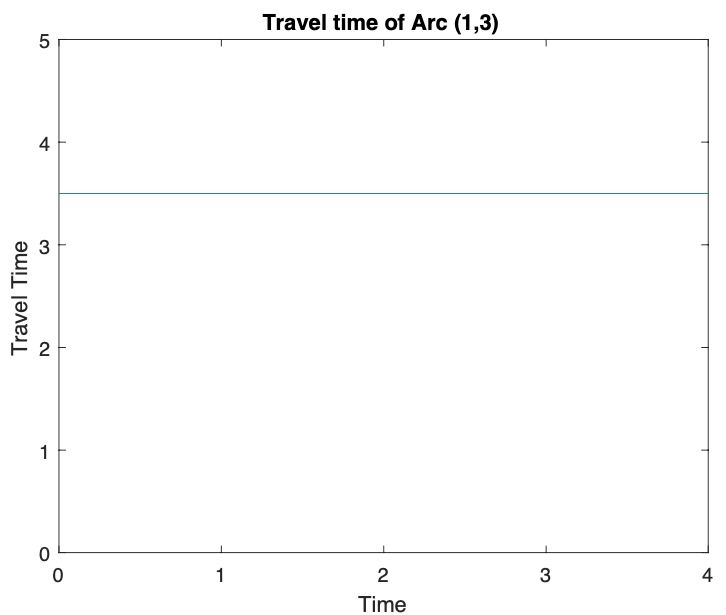
\includegraphics[width=.45\textwidth]{edited-images/Figure1c.jpg}}
\subcaptionbox{Cung \((2, 3)\)\label{fig:1d}}{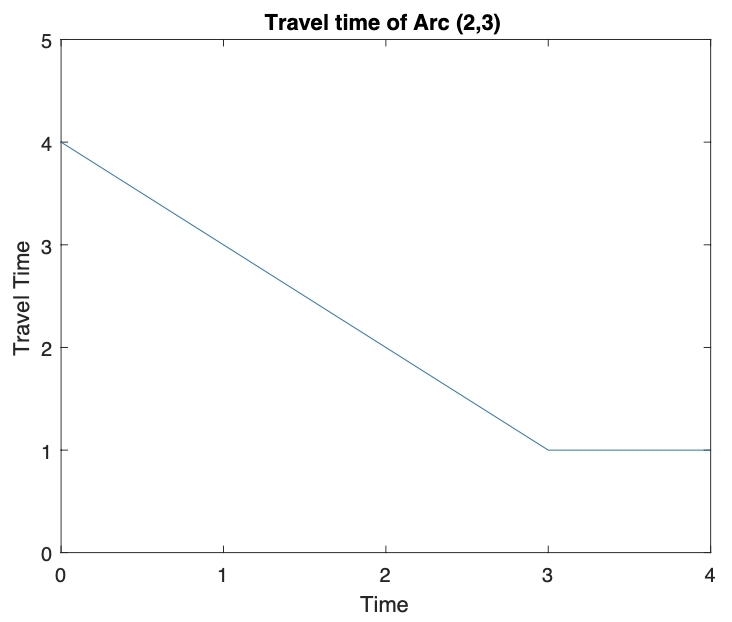
\includegraphics[width=.45\textwidth]{edited-images/Figure1d.jpg}}

\caption{Minh họa các hàm vận tốc}
\label{fig:1}
\end{figure}

Vì các hàm vận tốc có tính chất FIFO, khi giảm thời gian di
chuyển đến đích hoặc thời gian thực hiện, đường đi tối ưu luôn thỏa mãn
tính chất \(t_k + c_{i_k, i_{k+1}}(t_k) = t_{k+1}\) với
\(k = 1, \dots, m(P)-1\). Như đã đề cập ở trên, nghiệm tối ưu sẽ không
xuất hiện chờ đợi. Ngoài ra, khi giảm thời gian đến đích, đường đi tối
ưu sẽ có \(t_1^P = 0\).

Ba bài báo \cite{cooke1966shortest,orda1990shortest,dean2004shortest} đã đưa ra phương pháp
cho bài toán tìm đường đi đến đích sớm nhất có thể,  xuất phát tại đỉnh nguồn với thời gian cố định. 
Phương pháp này có độ phức tạp đa thức bằng cách mở rộng thuật toán tìm đường đi ngắn nhất
tiêu chuẩn. Điều tương tự áp dụng với bài toán tìm đường đi 
xuất phát từ nguồn muộn nhất có thể, đến đích với thời gian cố định.
\\
Bằng cách tính trước các hàm vận tốc \emph{đảo chiều}:

\begin{definition}
\label{id:reverse}  
Với
cạnh \((i, j)\) và thời gian \(t\), hàm \textbf{đảo chiều} được tính toán
tại \(t\) sẽ cho ra thời gian di chuyển \(\tau\) để kết quả thời gian
đến đỉnh \(j\) là \(t-\tau\). 
\end{definition}

Từ ý tưởng của \autoref{id:reverse} dẫn đến việc giải bài toán
TDSPP với nghiệm là đường đi ngắn nhất TDSP ở các phần sau.

\backmatter
\end{document}
% END DOCUMENT